\section{Sch1Objective\-Vector\-Traits Class Reference}
\label{classSch1ObjectiveVectorTraits}\index{Sch1ObjectiveVectorTraits@{Sch1ObjectiveVectorTraits}}
Inheritance diagram for Sch1Objective\-Vector\-Traits::\begin{figure}[H]
\begin{center}
\leavevmode
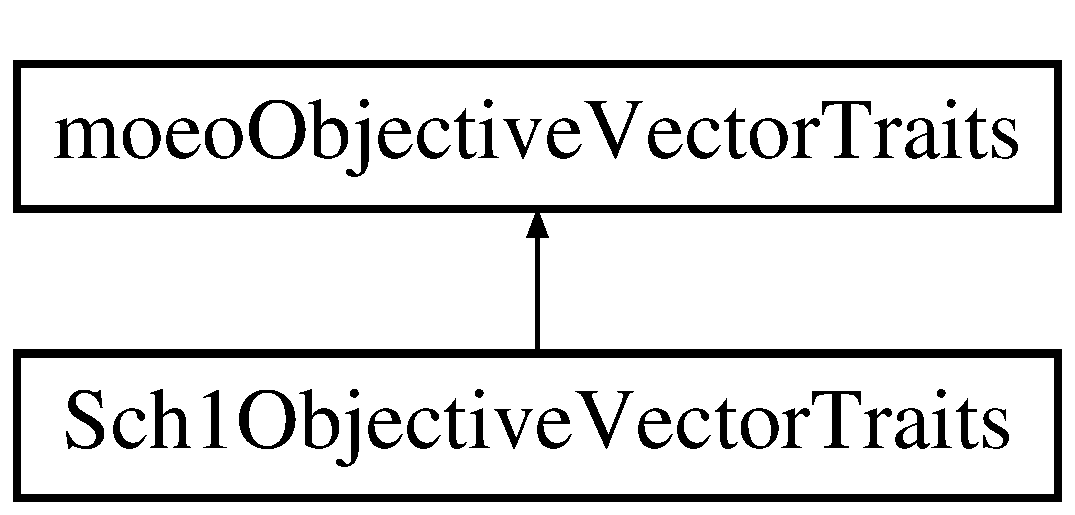
\includegraphics[height=2cm]{classSch1ObjectiveVectorTraits}
\end{center}
\end{figure}
\subsection*{Static Public Member Functions}
\begin{CompactItemize}
\item 
static bool \bf{minimizing} (int i)\label{classSch1ObjectiveVectorTraits_455ac35e419ad21c0a4ba4bbd2768ca5}

\item 
static bool \bf{maximizing} (int i)\label{classSch1ObjectiveVectorTraits_a7de212f3346dde550757e8a412baa4d}

\item 
static unsigned int \bf{n\-Objectives} ()\label{classSch1ObjectiveVectorTraits_54ae04aa8eb052223778ecae175be95b}

\begin{CompactList}\small\item\em Returns the number of objectives. \item\end{CompactList}\end{CompactItemize}


\subsection{Detailed Description}




Definition at line 21 of file Sch1.cpp.

The documentation for this class was generated from the following file:\begin{CompactItemize}
\item 
Sch1.cpp\end{CompactItemize}
